\chapter{Theoretical Background} % Main chapter title
\label{chap:Chapter2} % For referencing the chapter elsewhere, use \ref{Chapter1} 
\epigraph{''Let no one ignorant of geometry enter” }{\textit{Plato}}

O χώρος των \hyperref[abbr:WSN]{WSN} έχει και αυτός τα τελευταία χρόνια υψηλό ερευνητικό ενδιαφέρον.
Θα μπορούσε να πει κανείς - λόγο το ότι αποτελεί ένα πιο γενικό κλάδο - περισσότερο από ότι αυτό των 
drones. Συνεπώς θα μεταφερθούμε σε πρώτο επίπεδο στο πιο γενικό φάσμα, αυτό των \hyperref[abbr:WSN]{WSN} 
για να προσεγγίσουμε το localization problem. 

Όταν μιλάμε για \hyperref[abbr:WSN]{WSN}, αναφερόμαστε σε αυτόνομα ηλεκτρονικά συστήματα, χωρικά διασκορπισμένα σε ένα πεδίο - τα οποία συχνά περιλαμβάνουν
αισθητήρες και επικοινωνούν με τα γειτονικά τους ή σταθμούς βάσης για να μεταφέρουν πληροφορία \cite{wsn-wikipedia}.

Το καθένα από αυτά τα μεμονωμένα συστήματα ονομάζεται \textbf{Node}. Ενώ για το κάθε μεμονωμένο node 
μπορεί να έχουμε στην διάθεση μας location information ή όχι. 
Μία πρώτη σκέψη θα ήταν κάθε Node ενός συστήματος αισθητήρων να περιλαμβάνει \hyperref[abbr:GPS]{GPS} ώστε να γνωρίζουμε 
την θέση του. Αυτό μπορεί γρήγορα να καταρριφθεί σαν σκέψη, αν αναλογιστούμε ότι αρχικά το \hyperref[abbr:GPS]{GPS}
δεν είναι διαθέσιμο σε κάθε περιβάλλον λειτουργίας (π.χ. εσωτερικούς χώρους), όπως επίσης μπορεί να μην είναι δυνατή η χρήση του σε όλους τους κόμβους
ενός συστήματος, λόγο περιορισμών όπως το κόστος, μέγεθος του Node και energy consumption.   

\begin{table}[H]
    \caption{Nodes' names definitions}
    \label{tab:nodes-names-definition}
    \centering
    \begin{tabular}{ll}
        \toprule
        \textbf{Node name} & \textbf{Definition}  \\
        \midrule
            Unknown/Free/Dumb/Non-anchors & Their position is unknown \\
			Beacons/Anchors/Landmarks & Nodes with known location information \\
			Settled & Initial unknown nodes with estimated position \\
        \bottomrule
    \end{tabular}
\end{table}

Στην υπάρχουσα βιβλιογραφία \cite{wsn-Localization-systems} \cite{wsn-Localization-techniques} βρίσκουμε ότι
Nodes των οποίων η θέση είναι γνωστή ή άμεσα υπολογίσιμη, συχνά ονομάζονται \textbf{Beacons}. Πληροφορία σχετικά με την θέση αυτών
των Nodes είναι γνωστή, είτε γιατί έχουν τοποθετηθεί από εμάς σε προκαθορισμένες θέσεις, είτε μέσου ενός εξωτερικού συστήματος
όπως το \hyperref[abbr:GPS]{GPS}.
Αντίθετα κόμβοι για τους οποίους δεν έχουμε αρχικά πληροφορία της θέσης τους, ονομάζονται \textbf{Non-anchors}.
Άλλος ένας σημαντικός ορισμός, που θα πρέπει να αναφερθεί είναι ότι συχνά ονομάζουμε \textbf{Settle} nodes, 
αυτά τα οποία αρχικά δεν γνωρίζαμε την θέση τους αλλά στην συνέχεια την εκτιμήσαμε.
Στο table \ref{tab:nodes-names-definition} παρουσιάζονται συνοπτικά τα διάφορα ονόματα που έχουν δοθεί ανά 
καιρούς για το κάθε τύπο node.

Σκοπός ενός localization system είναι, με χρήση της γνώσης που έχουμε για τα beacon nodes να εκτιμήσουμε
την θέση όσο περισσότερων unknown nodes ώστε να τα μετατρέψουμε σε settled nodes και η εκτίμηση της κάθε
θέσης να είναι με όσο το δυνατόν μικρότερο error απόκλισης. 

\begin{figure} [H]
	\centering
	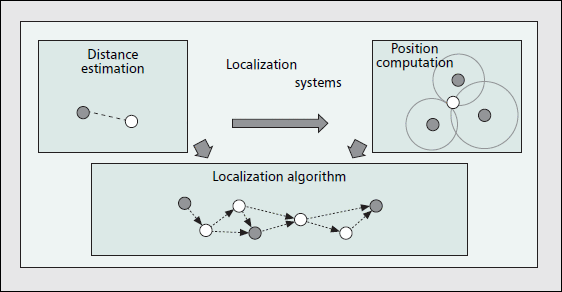
\includegraphics[scale=0.5]{Images/Theoretical-Background/localization-systems-components.png}
	\decoRule
	\caption[Localization System components]{Localization System components based on \cite{wsn-Localization-systems} (\href{https://ieeexplore.ieee.org/document/4407221}{URL})}
	\label{fig:Localization-Systems-components}
\end{figure}

Οι συγγραφείς του \cite{wsn-Localization-systems} επιχειρούν να χωρίσουν ένα localization system, ώστε 
αυτό να αποτελείται από τρία διακριτά components. Πρώτο μπορεί να θεωρηθεί αυτό του \textbf{Distance/Angle Estimation}, 
που σκοπό έχει να υπολογίσει την απόσταση ή γωνία που έχουν δύο nodes του συστήματος μεταξύ τους.
Η πληροφορία που θα παραχθεί από αυτό το component θα χρησιμοποιηθεί στα άλλα μέρη του συστήματος.
Στην συνέχεια υπάρχει το \textbf{Position Computation}, δουλειά του οποίου είναι να υπολογίσει την θέση ενός
node με βάση την γνώση που έχουμε για τα beacons και την πληροφορία που λάβαμε από το πρώτο component.
Ενώ τέλος είναι το κύριο μέρος του συστήματος, με όνομα \textbf{Localization Algorithm} και ουσιαστικά είναι
ο προκαθορισμένος τρόπος που θα ακολουθηθεί για να υπολογιστεί η θέση των unknown nodes με βάση όλες τις 
πληροφορίες που έχουμε.
Στο figure \ref{fig:Localization-Systems-components} δίνεται η απεικόνιση που έδωσαν οι συγγραφείς του 
\cite{wsn-Localization-systems} για να εξηγήσουν το παραπάνω. Ενώ στο figure \ref{fig:Localization-system}
έχει γίνει μία προσπάθεια να κατηγοριοποιηθούν τα κομμάτια καθώς και τεχνικές των Localization Systems,
με βάση τα \cite{wsn-Localization-systems} \cite{wsn-Localization-techniques} και αναλύονται στην συνέχεια
του κεφαλαίου.

\begin{figure} [H]
	\tikzset{
		basic/.style  = {draw, text width=2cm, font=\sffamily},
		root/.style   = {basic, thin, align=center, fill=white, text width=5cm},
		level 1/.style = {sibling distance=16em, level distance=5em},
		level-2/.style = {basic, thin, align=center, fill=white, text width=5.5cm},
		level-31/.style = {basic, thin, align=center, fill=white, text width=2cm},
		level-32/.style = {basic, thin, align=center, fill=white, text width=2.8cm},
		level-33/.style = {basic, thin, align=center, fill=white, text width=5cm},
		level-4/.style = {basic, thin, align=center, fill=white, text width=4.5cm},
		level-42/.style = {basic, thin, align=center, fill=white, text width=4.8cm},
		edge from parent/.style={->,solid,black,thick,draw}, 
		edge from parent path={(\tikzparentnode.south) -- (\tikzchildnode.north)},
		>=latex, node distance=1.5cm, edge from parent fork down
	}
	\centering
	\resizebox{1\textwidth}{!}{
		\begin{tikzpicture}[]
			\node[root] {\textbf{Localization Systems}}
				child {node[level-2] (c1) {\textbf{Distance/Angle Estimation}}}
				child {node[level-2] (c2) {\textbf{Position Computation}}}
				child {node[level-2] (c3) {\textbf{Localization Algorithm}}};
			
			% -----------------------------------------------------------------------------
			% Distance/Angle
			\node [level-31, below of = c1, xshift=-25pt] (c11) {Distance};
				\node [level-4, below of = c11, xshift=50pt] (c111) {Received Signal Strength};
				\node [level-4, below of = c111] (c112) {Lighthouse approach};
				\node [level-4, below of = c112] (c113) {Propagation time based measurements};
					\node [level-42, below of = c113, xshift=30pt] (c1131) {One-way propagation time};
					\node [level-42, below of = c1131] (c1132) {Roundtrip propagation time};
					\node [level-42, below of = c1132] (c1133) {Time Difference of Arrival};
					\foreach \value in {1,2,3} \draw[->] (c113.197) |- (c113\value.west);
				\foreach \value in {1,2,3} \draw[->] (c11.195) |- (c11\value.west);

			\node [level-31, below of = c1133, xshift=-80pt] (c12) {Angle};
				\node [level-4, below of = c12, xshift=70pt] (c121) {Receiver Antenna Amplitude response};
				\node [level-4, below of = c121] (c122) {Receiver antenna Phase response};
				\foreach \value in {1,2} \draw[->] (c12.210) |- (c12\value.west);
			\foreach \value in {1,2}   \draw[->] (c1.188) |- (c1\value.west);
			
			% Position Computation
			\node [level-32, below of = c2, xshift=25pt] (c21) {Trilateration};
			\node [level-32, below of = c21] (c22) {Bounding box};
			\node [level-32, below of = c22] (c23) {Triangulation};
			\node [level-32, below of = c23] (c24) {Multilateration};
			\node [level-32, below of = c24] (c25) {Probabilistic approaches};
			\node [level-32, below of = c25] (c26) {Central position};
			\foreach \value in {1,...,6} \draw[->] (c2.196) |- (c2\value.west);

			% Localization Algorithm
			\node [level-33, below of = c3, xshift=10pt] (c31) {Distributed/Centralized \\ Position Computation};
			\node [level-33, below of = c31] (c32) {With/Without Infrastructure};
			\node [level-33, below of = c32] (c33) {Relative/Absolute Positioning};
			\node [level-33, below of = c33] (c34) {Indoor/Outdoor scenarios};
			\node [level-33, below of = c34] (c35) {One-hop/Multihop};
			\foreach \value in {1,...,5} \draw[->] (c3.187) |- (c3\value.west);
		\end{tikzpicture}
	}
	\decoRule
	\caption[Localization-system-overview]{Localization system overview}
	\label{fig:Localization-system}
\end{figure}


%----------------------------------------------------------------------------------------
%	SECTION 1
%----------------------------------------------------------------------------------------
\section{Distance/Angle Estimation} \label{sec:Chapter2-1} 

\subsection{Distance}\label{sec:Chapter2-1-1}

Θα ξεκινήσουμε με μία σύντομη ανάλυση των τεχνικών που χρησιμοποιούνται ήδη 

\subsubsection{Received Signal Strength}
Η πρώτη τεχνική η οποία έχει χρησιμοποιηθεί για τον υπολογισμό απόστασης στα 
\hyperref[abbr:WSN]{WSN} είναι αυτή με όνομα Received Signal Strength Indicator
(\hyperref[abbr:RSSI]{RSSI}) και έχει ως αρχή την χρήση της έντασης ενός 
σήματος που λαμβάνουμε στον δέκτη, ως τρόπο υπολογισμού της απόστασης
του πομπό από αυτόν.


%-------------------------------------------
\cite{ideal-rssi-model}
Nowadays, this method is very popular
thanks to its simplicity and low implementation price be-
cause no additional hardware is required.


Also [4] and [5] discuss the
application of RSSI for distance measurements. They
conclude that it is not an appropriate metric for localization
systems because it lacks reliability between RSSI within
increasing distance in different directions from a trans-
mitter.

Path loss exponent η expresses how much
radio signal strength decreases with distance.

Received signal strength is measured from each
received frame as average value measured during the first
eight symbols (preamble) and converted to the RSS indi-
cator. This conversion is variable for every type of radio
chip [10].


With properly modeled path loss in a given envi-
ronment, it should be possible to formulate a relation
between distance and RSSI value.


Problems arise with
dynamical changes in environment because of radio signal
unstable properties.

Measurement accuracy of RSSI of the most today’s
radio chips used in sensor nodes is about ±4 dBm [11] and
RSSI is also rounded to integer values. This means that
notable uncertainty is brought to the estimation of distance.

Another uncertainty is caused by the signal propaga-
tion environment, like reflection, diffraction, scattering or
penetration of the radio signal through the objects.


Errors caused by hardware, signal propaga-
tion environment and errors caused by method for ap-
proximation of the RSSI value.

WSN devices used for RSS based method are not
suitable for distance estimation with high precision
%-------------------------------------------


%-------------------------------------------

%-------------------------------------------

\begin{figure} [H]
	\centering
	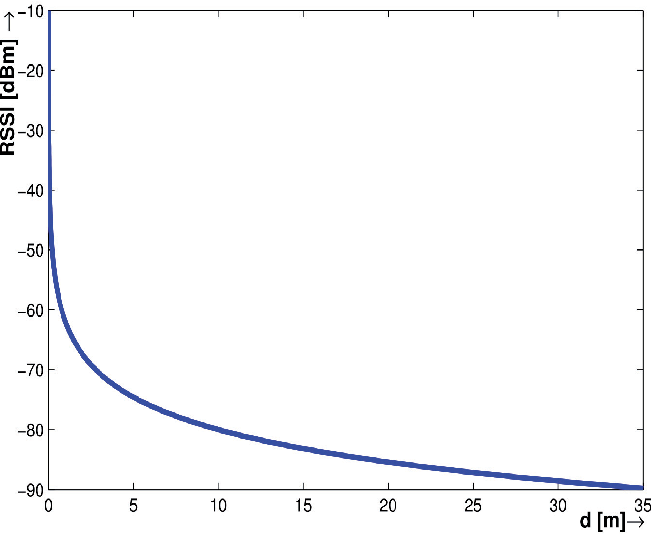
\includegraphics[scale=0.5]{Images/Theoretical-Background/Ideal-RSSI-over-distance.png}
	\decoRule
	\caption[Ideal RSSI over distance]{Ideal RSSI over distance based on \cite{ideal-rssi-model}}
	\label{fig:Ideal-RSSI-over-distance}
\end{figure}


\subsubsection{Propagation Time}
\subsubsection{Lighthouse}

\subsection{Angle}\label{sec:Chapter2-1-1}

%----------------------------------------------------------------------------------------
%	SECTION 2
%----------------------------------------------------------------------------------------
\section{Position Computation} \label{sec:Chapter2-2} 

%----------------------------------------------------------------------------------------
%	SECTION 3
%----------------------------------------------------------------------------------------
\section{Localization Algorithm} \label{sec:Chapter2-3} 

